% Research Note 03 -- Longer horizons, the trend band, and where traffic stops being "sunrise"
% Compile: pdflatex note03_horizons_and_trend.tex (run twice for refs)
% Figures in ./figures/: fig10 (multiweek), fig11 (multiyear trend), fig12 (seasonal stability).
\documentclass[11pt]{article}
\usepackage[margin=1in]{geometry}
\usepackage{amsmath,amssymb}
\usepackage{graphicx}
\usepackage{booktabs}
\usepackage{float}
\usepackage{xcolor}
\usepackage[colorlinks=true,linkcolor=blue,urlcolor=blue]{hyperref}
\graphicspath{{figures/}}

\newcommand{\veh}{\,\text{veh/h}}
\title{\textbf{Research Note 03}\\[2pt]
Longer Horizons, the Trend Band, and\\ Where Traffic Forecasting Stops Being ``Sunrise''}
\author{Traffic Forecasting Project}
\date{June 14, 2026}

\begin{document}
\maketitle

\begin{abstract}
\sloppy
\noindent
Notes 01--02 showed one-week-ahead flow forecasting is effectively solved by a
simple seasonal$+$holiday model ($R^2{=}0.949$): traffic, unlike asset prices, is
``sunrise-like'' -- dominated by a deterministic cycle anchored to human
schedules. This note asks what changes at \emph{longer} horizons. We frame the
signal as three frequency bands -- \emph{seasonal} (deterministic at any
horizon), \emph{noise} (bounded, averages out), and \emph{trend/level} (forecast
variance grows with horizon) -- and answer, in \emph{steady state}, at what
horizon the problem becomes interesting. The transition is a \textbf{smooth
onramp, not a sharp knee}: the ``copy recent weeks'' baseline degrades roughly
linearly as its data goes stale, from a $4\%$ gap to the floor at one week to
$13\%$ at four weeks and $25\%$ at twelve. By the natural threshold -- richer
level/trend
modeling recovering a holiday-scale margin -- the problem becomes interesting at
roughly \textbf{three to four weeks} out, and is unambiguously a trend problem by
about eight weeks. The cause is structural: across 2017--2021 the weekly \emph{shape}
is frozen (cross-year correlation $\ge0.99$) while the \emph{level} carries all
inter-temporal action; longer horizons just expose more of that slow level band.
(Regime breaks like COVID are the extreme tail of the same band -- a one-off, not
the everyday story.) We close on where richer statistical methods earn their keep.
\end{abstract}

\section*{Key findings}
\begin{itemize}
\item \textbf{Frequency-band view:} forecast difficulty is set by which band
  dominates. Seasonal is deterministic; noise averages out; only the trend band
  has horizon-growing uncertainty.
\item \textbf{A smooth onramp, no sharp knee.} The naive baseline's gap to the
  no-staleness floor grows $\sim$linearly: $4\%$ (1\,wk), $13\%$ (4\,wk), $25\%$
  (12\,wk). The steady-state problem becomes ``interesting'' (richer modeling
  recovers a holiday-scale margin) at \textbf{$H\approx3$--$4$ weeks}.
\item \textbf{Each week of horizon ages the level anchor.} A horizon-independent
  annual anchor stays flat while trailing data goes stale, so its optimal blend
  weight rises $0.20{\to}0.39$ over 1--12 weeks -- but it recovers only $\sim$half
  the gap; the rest needs genuine trend modeling.
\item \textbf{Seasonal shape is frozen; the level is everything.} 2017--2021
  weekly-shape cross-year correlation $\ge0.99$; the network level moves only with
  slow growth and the COVID shock ($240{\to}205{\to}228\veh$). Longer horizons
  simply expose more of the slow level band.
\item \textbf{Regime breaks are the tail, not the trend.} COVID spikes the
  one-week MAPE from $\sim$3.5\% to $\sim$60\% transiently -- a vivid one-off, but
  the everyday long-horizon difficulty is the smooth level drift above.
\end{itemize}

\section{A frequency-band view of forecast difficulty}
Write flow as $y_{i,t} = \underbrace{T_{i,t}}_{\text{trend/level}} +
\underbrace{S_{i,t}}_{\text{seasonal}} + \underbrace{\varepsilon_{i,t}}_{\text{noise}}$.
At forecast lead $h$ the three behave completely differently:
\begin{itemize}
\item \textbf{Seasonal} $S$ is anchored to the clock/calendar (hence to the sun):
  deterministic given the date, so it contributes \emph{zero} error at \emph{any}
  $h$. This is why short-horizon traffic is ``sunrise-like''.
\item \textbf{Noise} $\varepsilon$ (incidents, weather) is irreducible but bounded
  and, crucially, \emph{averages down} under aggregation -- the reason the
  weekly-aggregate MAPE is only $3.5\%$ (Note 02).
\item \textbf{Trend} $T$ is a near-random-walk: its forecast variance \emph{grows}
  with $h$. At one week it is negligible against $S$; at months--years it is the
  whole game.
\end{itemize}
The contrast with asset prices follows: a price is almost \emph{all} trend band
(no seasonal anchor) and its structure is arbitraged away, so it is hard even at
$h{=}1$. Traffic hands us a giant seasonal anchor that no one is incentivized to
arbitrage away -- so it is easy at short $h$, and only becomes price-like as the
horizon erodes the anchor's relative weight.

\section{The onramp: at what horizon does it get interesting?}
\label{sec:onramp}
A subtle constraint governs multi-week horizons. At lead $H$ weeks, a weekly lag
$k$ (weeks before the target) is observable only if $k\ge H$. So the ``copy recent
weeks'' baseline must use the four \emph{most recent available} weeks
$\{H,\dots,H+3\}$, which grow stale as $H$ grows: at $H{=}8$ the freshest usable
observation is two months old and may sit on the far side of a sub-annual
seasonal boundary (summer vs.\ back-to-school). All results here are pre-COVID
\emph{steady state} (test 2019), so this is the everyday behaviour, not a
regime-break artifact.

To separate staleness from irreducible error we add a horizon-\emph{independent}
floor: a \emph{centered oracle} that averages the weeks $\{\pm1,\pm2\}$ around the
target (it peeks at the future, so it has perfect concurrent level and no
staleness). Its RMSE is $38.1\veh$ ($R^2{=}0.946$) at \emph{every} horizon. The
gap between the naive baseline and this floor is exactly the prize a better
level/trend model could win. Figure~\ref{fig:sweep} and Table~\ref{tab:sweep}
trace it over $H=1,\dots,12$ weeks, alongside a simple recoverable model (an
optimal blend with a prior-year, calendar-aligned \emph{annual anchor}).

\begin{figure}[H]\centering
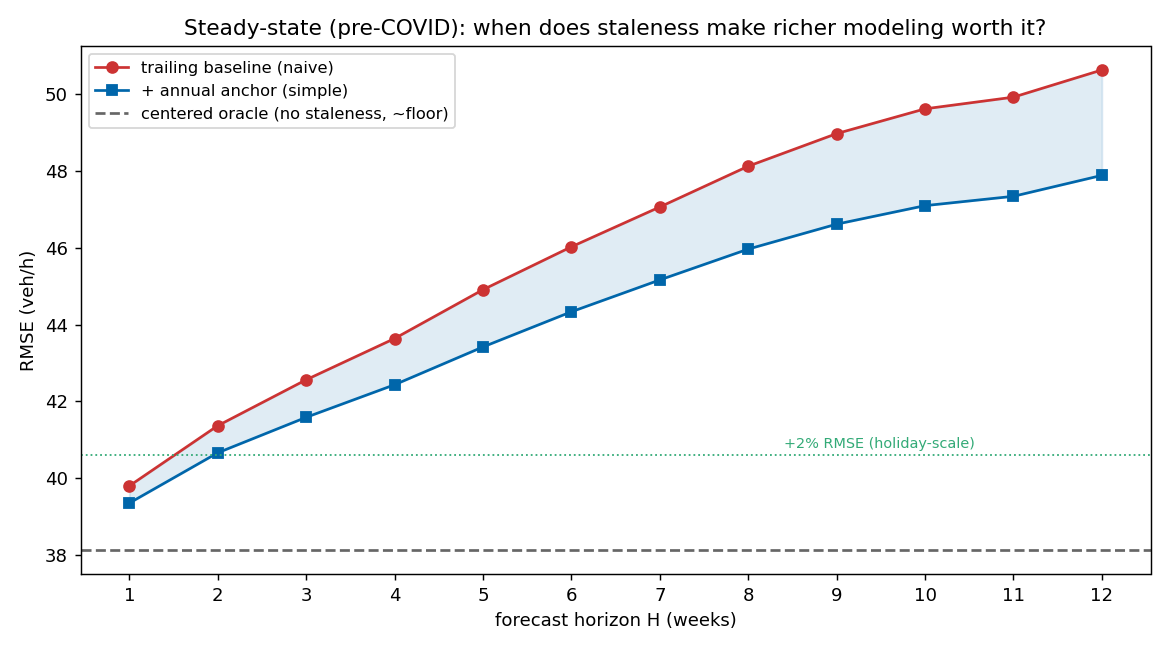
\includegraphics[width=0.92\linewidth]{fig13_horizon_sweep.png}
\caption{Steady-state RMSE vs.\ horizon. The naive baseline (red) pulls away from
the no-staleness floor (dashed) roughly linearly; the shaded band is the
recoverable prize. A simple annual anchor (blue) recovers about half of it; the
rest needs genuine trend modeling. ``Interesting'' (richer modeling worth a
holiday-scale margin) begins around $H{=}3$--$4$ weeks.}
\label{fig:sweep}
\end{figure}

\begin{table}[H]\centering
\caption{Steady-state horizon sweep (test 2019). Gap-to-floor is the share of RMSE
attributable to level staleness -- the target for richer modeling.}
\label{tab:sweep}
\begin{tabular}{cccc}
\toprule
Horizon & Naive RMSE & Gap to floor & Optimal annual weight \\
\midrule
1 week   & 39.8 & \phantom{0}4\% & 0.20 \\
2 weeks  & 41.4 & \phantom{0}8\% & 0.23 \\
4 weeks  & 43.6 & 13\% & 0.27 \\
8 weeks  & 48.1 & 21\% & 0.34 \\
12 weeks & 50.6 & 25\% & 0.39 \\
\bottomrule
\end{tabular}
\end{table}

The shape of the curve is the answer: there is \textbf{no sharp knee}. Each extra
week of horizon ages the anchor by one week and adds roughly constant level-drift
variance, so the gap-to-floor grows $\sim$linearly -- $4\%\to13\%\to25\%$ over
1--12 weeks. Reading off a threshold: below $\sim$2 weeks the naive rule is within
noise of the floor (solved); at $\mathbf{H\approx3\text{--}4}$ \textbf{weeks} the
recoverable gap reaches the scale of gains we already judged worth building (the
holiday model's $\sim$2\% RMSE), so a level/trend model starts to earn its keep;
by 8--12 weeks a quarter of the error is staleness and the naive rule is clearly
leaving accuracy on the table. The annual anchor -- nearly worthless at one week
(Note 02's YoY result) -- recovers an increasing share as it becomes
horizon-independent leverage, but only about \emph{half} the gap; closing the rest
needs an actual model of \emph{where we are in the year} and of the slow trend,
not a copy of recent weeks.

\section{The trend band: 2017--2021}
Zooming out to five years (Figure~\ref{fig:trend}) shows the decomposition
starkly. The network-mean level is nearly flat through early 2020 -- a slow,
gently growing trend with a tight seasonal oscillation on top -- and then falls
off a cliff at the March 2020 shelter-in-place order, partially recovering
through 2021.

\begin{figure}[H]\centering
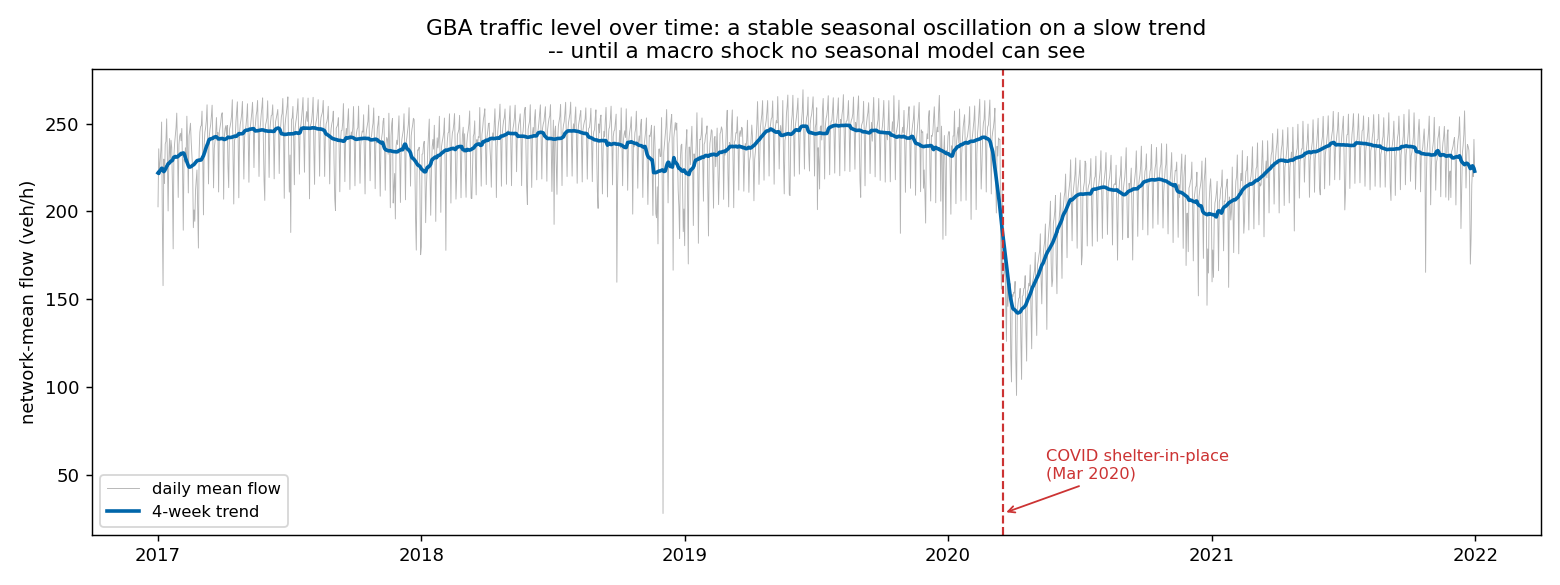
\includegraphics[width=\linewidth]{fig11_multiyear_trend.png}
\caption{Network-mean GBA flow, 2017--2021. A stable seasonal oscillation rides a
slow trend -- until a macro shock (COVID) that no seasonal model can anticipate.}
\label{fig:trend}
\end{figure}

Meanwhile the weekly \emph{shape} barely moves. Cross-year correlations of the
normalized weekly profile against 2019 are $0.9994$ (2017), $0.9994$ (2018),
$0.9953$ (2021) -- essentially frozen -- with mean levels
$239,237,241,205,228\veh$ for 2017--2021 (Figure~\ref{fig:stab}). Even 2020, the
exception, mostly drops the \emph{level} (and flattens the commute peaks under
remote work) while preserving the shape ($0.990$). The lesson:
\textbf{the seasonal band is boringly stable; essentially all the inter-temporal
action lives in the level/trend band}, and that band is where macro forces enter.

\begin{figure}[H]\centering
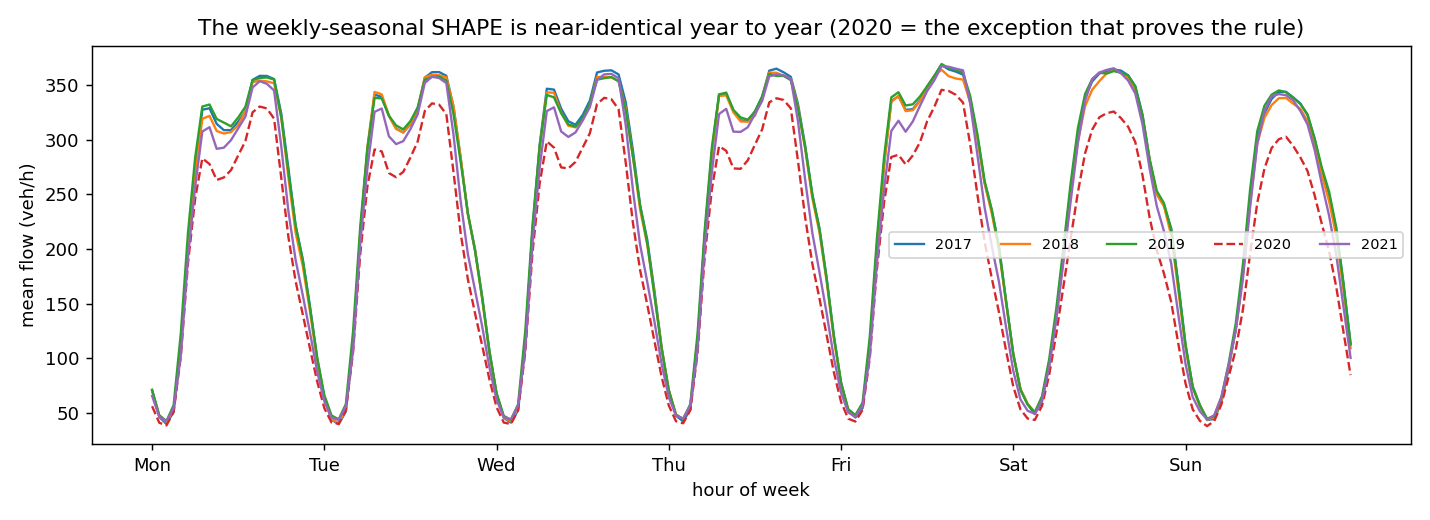
\includegraphics[width=\linewidth]{fig12_seasonal_stability.png}
\caption{The weekly-seasonal shape is near-identical year to year; 2020 (dashed)
drops the level and flattens the commute peaks but keeps the shape.}
\label{fig:stab}
\end{figure}

\subsection{The tail: regime breaks}
The COVID break is worth one paragraph not as the main story but as the
\emph{extreme tail} of the same level band. A trailing one-week-ahead forecaster
has a \emph{median} 2020 weekly-aggregate MAPE of $3.6\%$ -- normal! -- because
once the new regime persists for four weeks the trailing window re-adapts. But
\emph{at the transition} it fails catastrophically: the weeks of March~17 and
March~24, 2020 carry weekly MAPEs of $58\%$ and $60\%$ (a $16\times$ blowup),
decaying back over $\sim$4--6 weeks. Seasonal models do not see structural breaks;
they only recover from them. Such breaks are rare one-offs, but they share a
mechanism with the everyday onramp of \S\ref{sec:onramp}: both are the
\emph{level/trend band} asserting itself, gently as horizon grows and violently
when a macro shock hits. At horizons or in regimes where that band dominates,
traffic forecasting \emph{is} trend forecasting -- coupled to employment, fuel
prices, population, and remote-work structure -- and inherits their difficulty;
this is where the ``sunrise'' analogy gives way to the ``stock price'' one.

\section{Scope for richer statistical methods}
\label{sec:scope}
Does this leave room for methods beyond hand-crafted seasonal rules? The honest
answer from Notes 01--03: \textbf{model sophistication earns its keep when the
objective or the available information changes -- not on the original task.} On
one-week-ahead point forecasting of flow we proved the simple model sits at the
ceiling and ML on residuals adds nothing (Note 02). But four shifts open real
scope:

\begin{enumerate}
\item \textbf{Longer horizons $\Rightarrow$ trend modeling.} Forecasting the
  \emph{level} months--years out is a genuine, structured problem. State-space /
  structural time-series models (e.g.\ Bayesian structural time series, dynamic
  linear models), Gaussian processes, and models ingesting \emph{exogenous macro
  covariates} (employment, fuel price, population, remote-work indices) are the
  right tools -- and uncertainty grows with horizon, so they should be
  \emph{probabilistic}.
\item \textbf{Distributional targets $\Rightarrow$ uncertainty modeling.}
  Everything here was point accuracy, but much traffic value lives in the tails:
  $P(\text{severe congestion})$, calibrated prediction intervals, risk. The
  residual is strongly heteroscedastic (incident-driven heavy tails at peaks and
  transitions), which point rules ignore. Quantile regression, conditional
  density / distributional forecasting, and GARCH-type variance models have clear
  scope -- not for better means, but for calibrated risk.
\item \textbf{Robustness to regime change $\Rightarrow$ adaptive models.} The
  COVID failure motivates Markov-switching models, online change-point detection,
  and structural-time-series with explicit level-shift components -- which detect
  and adapt to breaks rather than merely recovering from them. The payoff is
  robustness, not average-case accuracy.
\item \textbf{Richer information $\Rightarrow$ learned global / spatial models.}
  Once genuinely new signal is added -- weather, events, network topology --
  models that capture nonlinear interactions and pool across sensors (gradient
  boosting, hierarchical Bayes, spatiotemporal graph networks) become
  appropriate. Spatial models specifically help \emph{short}-horizon incident
  nowcasting and missing-sensor imputation, where cross-corridor structure is
  real (it is not, at the week-ahead horizon -- Note 02).
\end{enumerate}

\paragraph{What we found when we tried.} We ran this ladder on the weekly level at
$H{=}4$--$8$ weeks: a recency rule (trailing mean of the most recent observable
weeks), a fitted classical model (deseasonalized Holt), a \emph{pooled} panel AR
with coefficients shared across all 2{,}352 sensors, and a trained global
gradient-boosted model. On \emph{endogenous} information the simplest rule is again
at the ceiling: the only thing that beats trailing is a one-parameter blend toward
the prior-year value, while the pooled AR (even with a smooth low-variance Fourier
seasonal) and the GBM \emph{under}perform it -- on a series $96\%$ predictable from
recency, ``estimate $+$ tiny shrinkage'' beats reconstructing the level from
components. One metric caution: the weekly-level $R^2$ ($\sim$0.96) is flattered by
the annual cycle in its denominator; the honest measures (RMSE, which grows $+47\%$
from one to six weeks, and skill over seasonal-naive) show the horizon effect that
$R^2$ hides.

\paragraph{Intrinsic or data-limited?} That verdict, though, rests on three
pre-COVID years of \emph{one} region -- and the level band is exactly where more
data could change it. Cross-regional co-movement (a common statewide level factor),
multi-year cycle/trend structure, and hierarchical shrinkage of noisy per-sensor
levels are all signals a larger panel could exploit and a single short region
cannot. The decisive cheap test is whether the deseasonalized level co-moves across
regions; if so, a forecastable common factor exists and pooling is warranted. So we
hold the ``rules win'' result as \emph{sample-limited}, not universal.

The unifying principle is the lesson of this project in miniature:
\textbf{complexity should follow information and objective, not precede them.}
The reason XGBoost lost on Note 02's task -- and pooled models lose here -- was an
information gap, not a modeling gap; change the task (longer horizon,
distributional, regime-robust) or the inputs (known-ahead covariates, more regions
and years) and the calculus flips. The most promising concrete next steps are
therefore (a) the cross-regional co-movement test and a pooled/hierarchical level
model, (b) known-ahead exogenous covariates (events, planned closures, calendar),
and (c) distributional forecasting for congestion risk -- each targeting value the
seasonal baseline structurally cannot reach.

\paragraph{Reproducibility.} Figures and numbers from \texttt{src/}:
\texttt{horizon\_sweep} (\S3, fig.\,13, the steady-state onramp),
\texttt{multiyear\_trend} (\S4, figs.\,11--12, and the COVID-transition
quantification inline), with \texttt{multiweek\_horizon} as the coarse precursor.

\end{document}
